\documentclass[12pt]{beamer}

\usepackage[brazil]{babel}
\usepackage[utf8]{inputenc}
\usepackage[T1]{fontenc}
\usepackage{animate}
\usepackage{amsbsy}
\usepackage{amsfonts}
\usepackage{amsmath}
\usepackage{amssymb}
\usepackage{amsthm}
\setbeamertemplate{theorems}[numbered] % to number
\usepackage[toc,page,title,titletoc]{appendix}
\usepackage{dsfont}
\usepackage{esvect}
\usepackage[labelfont=bf]{caption}
%\usepackage{subcaption}
\usepackage{float}
\usepackage[Glenn]{fncychap}%Sonny %Conny %Lenny %Glenn %Renje %Bjarne %Bjornstrup
\usepackage{graphicx}
\usepackage{subfig}
\usepackage{indentfirst}%Para indentar os paragrafos automáticamente
\usepackage{lipsum}
\usepackage{longtable}
\usepackage{mathtools}
\usepackage{listings}%Inserir codigo do R no latex
\usepackage{multirow}
\usepackage{multicol}
\usepackage{csquotes}
\usepackage[maxcitenames=2,terseinits=true,natbib=true, style=authoryear, maxbibnames=99]{biblatex}
\addbibresource{../Referencias/Referencias.bib}
\usepackage[figuresright]{rotating}
\usepackage{spalign}
\usepackage{pgfplots}
\pgfplotsset{compat=1.17}
\usepackage{tikz}
\usepackage{fontawesome}
\usepackage{color, colortbl}
\usepackage{url}
\usepackage{cancel}
\usepackage{accents}
\usepackage{bm}
\usepackage{ragged2e}%para justificar o texto dentro de algum ambiente
\definecolor{Gray}{gray}{0.9}
\definecolor{LightCyan}{rgb}{0.88,1,1}


\usepackage[all]{xy}
\usepackage{hyperref,bookmark}
\hypersetup{
  colorlinks=true,
  linkcolor=blue,
  citecolor=red,
  filecolor=blue,
  urlcolor=blue,
}

\usetheme{Madrid}
\usecolortheme[RGB={193,0,0}]{structure}

%\setbeamertemplate{footline}[frame number]
%\setbeamertemplate{footline}[text line]{%
%  \parbox{\linewidth}{\vspace*{-8pt}\hfill\date{}\hfill\insertshortauthor\hfill\insertpagenumber}}
\beamertemplatenavigationsymbolsempty
\renewcommand{\vec}[1]{\mbox{\boldmath$#1$}}
\newtheorem{Teorema}{Teorema}
\newtheorem{Proposicao}{Proposição}
\newtheorem{definicao}{Definição}
\newtheorem{Corolario}{Corolário}
\newtheorem{Demonstracao}{Demonstração}
\newcommand{\bx}{\ensuremath{\bar{x}}}
\newcommand{\Ho}{\ensuremath{H_{0}}}
\newcommand{\Hi}{\ensuremath{H_{1}}}
\newcommand{\at}[2][]{#1|_{#2}}
\newcommand\xuparrow[1][2ex]{%
   \mathrel{\rotatebox{-90}{$\xleftarrow{\rule{#1}{0pt}}$}}
}
\apptocmd{\frame}{}{\justifying}{} % Allow optional arguments after frame.

\makeatletter
\setbeamertemplate{footline}
{
  \leavevmode%
  \hbox{%
  \begin{beamercolorbox}[wd=.3\paperwidth,ht=2.25ex,dp=1ex,center]{author in head/foot}%
    \usebeamerfont{author in head/foot}\mytext
  \end{beamercolorbox}%
  \begin{beamercolorbox}[wd=.3\paperwidth,ht=2.25ex,dp=1ex,center]{title in head/foot}%
    \usebeamerfont{title in head/foot}\mytextt
  \end{beamercolorbox}%
  \begin{beamercolorbox}[wd=.35\paperwidth,ht=2.25ex,dp=1ex,right]{site in head/foot}%
    \usebeamerfont{site in head/foot}\mytexttt\hspace*{2em}
    \insertframenumber{} / \inserttotalframenumber\hspace*{2ex} 
  \end{beamercolorbox}}%
  \vskip0pt%
}
\makeatother

\providecommand{\arcsin}{} \renewcommand{\arcsin}{\hspace{2pt}\textrm{arcsen}}
\providecommand{\sin}{} \renewcommand{\sin}{\hspace{2pt}\textrm{sen}}
\newcommand{\N}{\rm I\!N}
\newcommand{\I}{\rm I\!I}
\newcommand{\R}{\rm I\!R}
\newcommand{\Sim}{\overset{\text{iid}}{\sim}}
\newcommand{\Lim}{{\displaystyle \lim_{n\to\infty}}}
\newcommand{\LimInf}{{\displaystyle \liminf_{n\to\infty}}}
\newcommand{\rightLim}{\xrightarrow[n\rightarrow\infty]{}}
\newcommand{\Sumi}{{\displaystyle \sum_{i=1}^{n}}}
\newcommand{\Int}{{\displaystyle \int_{-\infty}^{+\infty}}}
\newcommand{\ConvD}{\overset{D}{\rightarrow}}
\newcommand{\ConvP}{\overset{P}{\rightarrow}}
\newcommand{\Prodi}{{\displaystyle \prod_{i=1}^{n}}}
\newcommand{\SetaUP}[2]{\underset{\mathclap{\substack{\xuparrow[30pt] \\ #1}}}{#2}}
%\newcommand{\SetaInclinada}[2]{\underset{\mathclap{\substack{\rotatebox{135}{\xuparrow[30pt] \\ #1}}}}{#2}}
\newcommand{\Home}{\begin{tikzpicture}
\node[scale=2] at (3,4) {\text{Para}~\faHome};
\end{tikzpicture}}
\newcommand{\vecX}{\boldsymbol{X}}
\newcommand{\Implica}[1]{\xRightarrow{#1}}
\newcommand{\SeSe}{\iff}
\newcommand{\EscoreA}{\dfrac{\partial}{\partial\theta}\log{f(x,\theta)}}
\newcommand{\EscoreB}{\dfrac{\partial^{2}}{\partial\theta^{2}}\log{f(x,\theta)}}
\newcommand{\cqd}{\text{cqd}~\blacksquare}
\newcommand{\seqX}{$X_{1},\ldots,X_{n}$}
\newcommand{\seqY}{$Y_{1},\ldots,Y_{n}$}
\newcommand{\tend}[1]{\hbox{\oalign{$\bm{#1}$\crcr\hidewidth$\scriptscriptstyle\bm{\sim}$\hidewidth}}}

%\newtheorem{Teorema}{Teorema}
%\newtheorem{Proposicao}{Proposição}
%\newtheorem{Definicao}{Definição}
%\newtheorem{Corolario}{Corolário}
%\newtheorem{Demonstracao}{Demonstração}

\titlegraphic{\hspace*{8cm}\href{https://fsbmat-ufv.github.io/}{
\includegraphics[width=2cm]{figs/mylogo.png}}
}

%Continuar a numeracao em slides diferentes
\newcounter{saveenumi}
\newcommand{\seti}{\setcounter{saveenumi}{\value{enumi}}}
\newcommand{\conti}{\setcounter{enumi}{\value{saveenumi}}}

\resetcounteronoverlays{saveenumi}

% Layout da pagina
\hypersetup{pdfpagelayout=SinglePage}

%Para o \pause funcionar dentro do ambiente align
\makeatletter
\let\save@measuring@true\measuring@true
\def\measuring@true{%
  \save@measuring@true
  \def\beamer@sortzero##1{\beamer@ifnextcharospec{\beamer@sortzeroread{##1}}{}}%
  \def\beamer@sortzeroread##1<##2>{}%
  \def\beamer@finalnospec{}%
}
\makeatother
\setLayoutColor{3} 

\title{Inferência Estatística II}
\author{Prof. Fernando de Souza Bastos\texorpdfstring{\\ fernando.bastos@ufv.br}{}}
\institute{Departamento de Estatística\texorpdfstring{\\ Programa de Pós-Graduação em Estatística Aplicada e Biometria}\texorpdfstring{\\ Universidade Federal de Viçosa}{}\texorpdfstring{\\ Campus UFV - Viçosa}{}}
\date{}
\newcommand\mytext{Aula 15}
\newcommand\mytextt{Fernando de Souza Bastos}
\newcommand\mytexttt{\url{https://est711.github.io/}}


\begin{document}
%\SweaveOpts{concordance=TRUE}

\frame{\titlepage}

\begin{frame}{}
\frametitle{\bf Sumário}
\tableofcontents
\end{frame}

\section{Introdução}
\begin{frame}{}
\begin{block}{}
\justifying
Considere $X_1, \ldots, X_n$ variáveis aleatórias independentes e identicamente distribuídas com função de densidade de probabilidade $f(x; \theta)$ para $\theta \in \Omega$. Considere, ainda, as hipóteses bilaterais:

\[
H_0: \theta = \theta_0 \quad \text{versus} \quad H_1: \theta \neq \theta_0
\]

em que $\theta_0$ é um valor especificado. Lembre-se de que a função de verossimilhança e seu logaritmo são dados por:

\begin{align*}
L(\theta) = \prod_{i=1} f(X_i; \theta)~\text{e}~ \ell(\theta) = \sum_{i=1} \log f(X_i; \theta)
\end{align*}

Com $\hat{\theta}$ sendo a estimativa de máxima verossimilhança de $\theta$.
\end{block}
\end{frame}

\begin{frame}{}
\begin{block}{}
\justifying
Sabemos, que se $\theta_0$ é o valor verdadeiro de $\theta$, então, assintoticamente, $L(\theta_0)$ é o valor máximo de $L(\theta)$. Considere a razão de duas funções de verossimilhança, a saber,

\begin{align}\label{razao1}
    \Lambda = \frac{L(\theta_0)}{L(\hat{\theta})},~\hat{\theta}\in\Theta.
\end{align}
\end{block}
\pause 
\begin{block}{}
\justifying
Observe que $\Lambda \leq 1,$ pois $L(\theta_{0})$ é uma verossimilhança restrita a $\Theta_{0}$ e $L(\hat{\theta})$ é uma verossimilhança irrestrita a $\Theta.$ Assim, se $\theta_{0}$ é o verdadeiro valor do parâmetro, $L(\hat{\theta})$ atingirá $L(\theta_{0})$ e $\Lambda=1,$ caso contrário, $L(\theta_{0})<L(\hat{\theta})$ e $\Lambda < 1.$
\end{block}
\end{frame}

\section{Teste da Razão de Verossimilhança}
\begin{frame}{}
\begin{block}{}
\justifying
Para um nível de significância especificado $\alpha$, isso leva à regra de decisão intuitiva:

\begin{center}
Rejeitar $H_0$ em favor de $H_1$ se $\Lambda \leq c,$
\end{center}

em que $c$ é tal que $\alpha = P_{\theta_0}(\Lambda \leq c)$. Chamamos isso de teste da razão de verossimilhança (TRV).
\end{block}
\end{frame}

\section{Exemplo 1 - Hipóteses Bilaterais}
\begin{frame}{Exemplo 1 - Hipóteses Bilaterais}
	\begin{block}{}
			\justifying
		Considere uma amostra aleatória \(X_1, X_2, X_3\) de uma distribuição normal \(N(\theta, 1)\). Desejamos testar as hipóteses:
		
		\[
		H_0: \theta = 5 \quad \text{versus} \quad H_1: \theta \neq 5,
		\]
		
		e os dados observados \(X_1 = 6\), \(X_2 = 5\), \(X_3 = 7\).		
	\end{block}
\end{frame}

\begin{frame}
	\begin{block}{}

			Para \(n = 3\), a função de verossimilhança conjunta é:
			\[
			L(\theta) = \prod_{i=1}^3 \frac{1}{\sqrt{2\pi}} \exp\left(-\frac{(X_i - \theta)^2}{2}\right).
			\]
			
			\begin{itemize}
				\item Sob \(H_0\), temos \(\theta = \theta_0 = 5\).
				\item Sob \(H_1\), o estimador de máxima verossimilhança é \[\hat{\theta} = \bar{X} = \frac{1}{3}(6 + 5 + 7) = 6\].
			\end{itemize}
			
	\end{block}
\end{frame}

\begin{frame}
	\begin{block}{}
Substituímos \(\theta_0\) e \(\hat{\theta}\) na função de verossimilhança:
		\[
		\Lambda = \frac{L(\theta_0)}{L(\hat{\theta})}\Rightarrow 
		-2 \ln \Lambda = 2 \sum_{i=1}^3 \frac{(X_i - \theta_0)^2 - (X_i - \hat{\theta})^2}{2}.
		\]
		
		Ao considerar os dados:
		\[
		\Lambda=e^{-\frac{3}{2}}\Rightarrow -2 \ln \Lambda = 3.
		\]
	\end{block}
\end{frame}

\begin{frame}
	\begin{block}{}
	\justifying
		\textbf{Regra de Decisão:} Sob \(H_0\), a estatística \(-2 \ln \Lambda\) segue uma distribuição \(\chi^2(1)\). Para um nível de significância \(\alpha = 0,05\), o valor crítico é:
		\[
		\chi^2_{0,05}(1) = 3,841.
		\]
		
		Como \(-2 \ln \Lambda = 3 < 3,841\), não rejeitamos \(H_0\).

	
	Com os dados \(X_1 = 6\), \(X_2 = 5\), \(X_3 = 7\), há evidência suficiente para não rejeitar \(H_0\) e aceitar que \(\theta = 5\) ao nível de significância de 5\%.	
	\end{block}
\end{frame}

\begin{frame}{Exemplo 2 - Hipóteses Unilaterais}
	\begin{block}{}
			\justifying
	Considere uma amostra aleatória \(X_1, X_2, X_3\) de uma distribuição normal \(N(\theta, 1)\). Desejamos testar as hipóteses:
	
	\[
	H_0: \theta \leq 5 \quad \text{versus} \quad H_1: \theta > 5,
	\]
	
	e os dados observados \(X_1 = 6\), \(X_2 = 5.5\), \(X_3 = 6.5\).
			
	\end{block}
\end{frame}

\begin{frame}
	\begin{block}{}
		\justifying
		Para \(n = 3\), a função de verossimilhança conjunta é:
			\[
			L(\theta) = \prod_{i=1}^3 \frac{1}{\sqrt{2\pi}} \exp\left(-\frac{(X_i - \theta)^2}{2}\right).
			\]
			
			\begin{itemize}
				\item Sob \(H_0: \theta \leq \theta_0\), o valor de \(\theta\) que maximiza a verossimilhança é \(\hat{\theta}_0 = \theta_0 = 5\).
				\item Sob \(H_1: \theta > \theta_0\), o estimador de máxima verossimilhança é \(\hat{\theta} = \bar{X} = \frac{1}{3}(6 + 5.5 + 6.5) = 6\).
			\end{itemize}
		
	\end{block}
\end{frame}

\begin{frame}
	\begin{block}{}
Substituímos \(\hat{\theta}_0\) e \(\hat{\theta}\) na função de verossimilhança:
			\[
			\Lambda = \frac{L(\hat{\theta}_0)}{L(\hat{\theta})}\Rightarrow 
			-2 \ln \Lambda = 2 \sum_{i=1}^3 \frac{(X_i - \hat{\theta}_0)^2 - (X_i - \hat{\theta})^2}{2}.
			\]
			
			Para os dados:
			\[
			-2 \ln \Lambda = 3
			\]

	\end{block}
\end{frame}

\begin{frame}
	\begin{block}{}
		\justifying
\textbf{Regra de Decisão:} Sob \(H_0\), a estatística \(-2 \ln \Lambda\) segue uma distribuição qui-quadrado com 1 grau de liberdade (\(\chi^2(1)\)). Para um nível de significância \(\alpha = 0,05\), o valor crítico é:
			\[
			\chi^2_{0,05}(1) = 3,841.
			\]
			
			Como $\bar{X}>\theta_{0}=5,$ e \(-2 \ln \Lambda = 3 < 3,841\), não rejeitamos \(H_0\). Com os dados \(X_1 = 6\), \(X_2 = 5,5\), \(X_3 = 6,5\), não há evidência suficiente para rejeitar \(H_0\) ao nível de significância de 5\%.	
	\end{block}
\end{frame}

\begin{frame}{Exemplo 2 - Hipóteses Unilaterais}
	\begin{block}{Regra de Decisão}
		\justifying
		Sob \(H_0: \theta \leq 5\), considere a estatística de teste:
		\[
		-2 \ln \Lambda.
		\]
		Para rejeitar \(H_0\):
		\begin{enumerate}
			\item Verifique a direção do desvio:
			\begin{itemize}
				\item Se \(\hat{\theta} \leq \theta_0\), não rejeite \(H_0\).
				\item Caso contrário, passe para o próximo passo.
			\end{itemize}
			\item Compare \(-2 \ln \Lambda\) com o valor crítico:
			\[
			\chi^2_{0.05}(1) = 3.841.
			\]
			\item Rejeite \(H_0\) se \(-2 \ln \Lambda > 3.841\).
		\end{enumerate}
	\end{block}
\end{frame}

\begin{frame}{Exemplo 1 - Hipóteses Bilaterais}
	\begin{block}{}
		\justifying
		Considere as hipóteses:
		\[
		H_0: \theta = \theta_{0} \quad \text{versus} \quad H_1: \theta \neq \theta_{0}.
		\]
		
		\textbf{Características:}
		\begin{itemize}
			\justifying
			\item O teste avalia se o parâmetro \(\theta\) é exatamente igual a \(\theta_{0}\) ou se difere em qualquer direção (maior ou menor).
			\item A função de verossimilhança considera desvios em ambas as direções (\(\theta > \theta_{0}\) ou \(\theta < \theta_{0}\)).
		\end{itemize}
		
		\textbf{Região Crítica:}
		\begin{itemize}
			\justifying
			\item Rejeitamos \(H_0\) se a estatística do teste \(-2 \ln \Lambda\) for maior que o valor crítico, indicando que \(\theta\) está longe de \(\theta_{0}\) em qualquer direção.
		\end{itemize}
	\end{block}
\end{frame}

\begin{frame}{Exemplo 2 - Hipóteses Unilaterais}
	\begin{block}{}
		\justifying
		Considere as hipóteses:
		\[
		H_0: \theta \leq \theta_{0} \quad \text{versus} \quad H_1: \theta > \theta_{0}.
		\]
		
		\textbf{Características:}
		\begin{itemize}
			\justifying
			\item O teste avalia se o parâmetro \(\theta\) é maior que \(\theta_{0}\), contra a hipótese de que \(\theta\) seja menor ou igual a \(\theta_{0}\).
			\item A função de verossimilhança considera apenas desvios positivos (\(\theta > \theta_{0}\)).
		\end{itemize}
		
		\textbf{Região Crítica:}
		\begin{itemize}
			\justifying
			\item Rejeitamos \(H_0\) se a estatística do teste \(-2 \ln \Lambda\) for maior que o valor crítico, indicando que há evidência de que \(\theta > \theta_{0}\).
		\end{itemize}
	\end{block}
\end{frame}

\begin{frame}{Resumo - Diferença na Região Crítica}
	\begin{block}{Exemplo 1 - Bilateral}
		\justifying
		\begin{itemize}
			\justifying
			\item Considera desvios em ambas as direções (\(\theta > \theta_{0}\) ou \(\theta < \theta_{0}\)).
			\item Mais rigoroso, pois rejeita \(H_0\) desvios significativos em qualquer direção.
		\end{itemize}
	\end{block}
	\begin{block}{Exemplo 2 - Unilateral}
		\justifying
		\begin{itemize}
			\item Considera apenas desvios em uma direção específica (\(\theta > \theta_{0}\)).
			\item Mais sensível a mudanças direcionais, rejeitando \(H_0\) se houver forte evidência de \(\theta > \theta_{0}\).
		\end{itemize}
	\end{block}
\end{frame}

\begin{frame}{Exemplo 3 - Hipóteses Bilaterais}
	\begin{block}{}
		\justifying
		Considere uma amostra aleatória $X_1, X_2, \ldots, X_n$ de uma distribuição $N(\theta, \sigma^2)$, em que $-\infty < \theta < \infty$ e $\sigma^2 > 0$ são conhecidos. Vamos considerar as hipóteses:
		
		\[ H_0 : \theta = \theta_0 \quad \text{versus} \quad H_1 : \theta \neq \theta_0, \]
		
		em que $\theta_0$ é especificado. A função de verossimilhança é dada por:
		
		
		\begin{align}
			L(\theta) &= \left(\frac{1}{2\pi\sigma^2}\right)^{n/2} \exp\left\{ -\frac{1}{2\sigma^2} \sum_{i=1}^{n}(x_i - \theta)^2 \right\} \\
			&= \left(\frac{1}{2\pi\sigma^2}\right)^{n/2} \exp\left\{ -\frac{1}{2\sigma^2} \sum_{i=1}^{n}(x_i - \bar{x})^2 \right\} \exp\left\{ -\frac{1}{2\sigma^2}n(\bar{x} - \theta)^2 \right\},
		\end{align}
		
	\end{block}
\end{frame}

\begin{frame}{}
	\begin{block}{}
		\justifying
		Em $\Omega = \{\theta : -\infty < \theta < \infty\}$, o estimador de máxima verossimilhança é $\hat{\theta} = \bar{x}$, e, portanto, a razão de verossimilhança é:
		
		\[
		\begin{aligned}
			\Lambda &= \frac{L(\theta_0)}{L(\hat{\theta})} \\
			&= \exp\left\{ -\frac{1}{2\sigma^2}n(\bar{X} - \theta_0)^2 \right\}.
		\end{aligned}
		\]
	\end{block}
	\pause
	\begin{block}{}
		\justifying
		Logo, $\Lambda \leq c$ é equivalente a $-2 \log \Lambda \geq -2 \log c$. No entanto, 
		\[
		-2 \log \Lambda = \left(\frac{\Bar{X} - \theta_0}{\sigma/\sqrt{n}}\right)^{2},
		\]
		que segue uma distribuição $\chi^2(1)$ sob $H_0$. 
	\end{block}
\end{frame}


\begin{frame}{}
	\begin{block}{}
		\justifying
		Portanto, o teste da razão de verossimilhança com nível de significância $\alpha$ afirma que rejeitamos $H_0$ e aceitamos $H_1$ quando
		\[
		\left(\frac{\Bar{X} - \theta_0}{\sigma/\sqrt{n}}\right)^{2} \geq \chi^2_\alpha(1).
		\]
		
		%Observe que este teste é o mesmo que o teste $z$ para uma média normal discutido anteriormente, com $s$ substituído por $\sigma$. Portanto, a função poder para este teste é dada na expressão:
		%\begin{align*}
		%\gamma(\mu) &= P\left(\Bar{X} \leq \mu_0 - \frac{z_{\alpha/2}\sigma}{\sqrt{n}}\right) + P\left(\Bar{X} \geq \mu_0 + \frac{z_{\alpha/2}\sigma}{\sqrt{n}}\right)\\ 
		%&= \Phi\left(\frac{\sqrt{n}(\mu_0 - \mu)}{\sigma} - z_{\alpha/2}\right) + 1 - \Phi\left(\frac{\sqrt{n}(\mu_0 - \mu)}{\sigma} + z_{\alpha/2}\right)
		%\end{align*}
	\end{block}
	\pause
		\begin{block}{}
		
		\begin{itemize}
			\justifying
			\item O teste baseado na estatística
			\[
			\left(\frac{\bar{X} - \theta_0}{\sigma / \sqrt{n}}\right)^2
			\]
			é equivalente ao teste \(z\)-bilateral porque:
			\begin{enumerate}
				\justifying
				\item Ele utiliza o quadrado da estatística \(z\), que naturalmente segue uma distribuição \(\chi^2(1)\) sob \(H_0\).\pause
				\item A bilateralidade está embutida no quadrado da estatística, o que elimina a necessidade de dividir o nível de significância \(\alpha\) entre as duas caudas.
			\end{enumerate}
		\end{itemize}
	\end{block}
\end{frame}

\begin{frame}{}
	\begin{block}{}

		\begin{itemize}		
			\justifying
			\item A razão para usarmos \(\chi^2_\alpha(1)\) em vez de \(\chi^2_{\alpha/2}(1)\) é:
			\begin{enumerate}
				\justifying
				\item A estatística \(-2 \ln \Lambda\) segue uma distribuição qui-quadrado com 1 grau de liberdade, que já reflete a probabilidade acumulada na cauda superior.\pause
				\item A bilateralidade está implícita porque a estatística considera apenas o quadrado das diferenças (\((\bar{X} - \theta_0)^2\)), incorporando desvios para ambos os lados de \(\theta_0\).\pause
				\item No caso da estatística \(Z^2 \sim \chi^2(1)\), rejeitamos \(H_0\) quando:
				\[
				Z^2 \geq \chi^2_\alpha(1),
				\]
				o que é equivalente a:
				\[
				|Z| \geq \sqrt{\chi^2_\alpha(1)}.
				\]
			\end{enumerate}
		\end{itemize}
	\end{block}
\end{frame}



\section{Exemplo 2: Distribuição Exponencial}
\begin{frame}{Teste da Razão de Verossimilhança para a Distribuição Exponencial}
\begin{block}{}
\justifying
Suponha que $X_1, \ldots, X_n$ são variáveis i.i.d com densidade de probabilidade

\[
f(x; \theta) = \theta^{-1} e^{-x/\theta}, \quad \text{para} \quad x, \theta > 0
\]

As hipóteses são dadas por 
\[
H_0: \theta = \theta_0 \quad \text{versus} \quad H_1: \theta \neq \theta_0.
\]

A função de verossimilhança pode ser escrita como:

\[
L(\theta) = \theta^{-n} e^{-n\Bar{X}/\theta}
\]

É fácil ver que a estimativa de máxima verossimilhança de $\theta$ é $\Bar{X}.$
\end{block}
\end{frame}

\begin{frame}{}
\begin{block}{}
\justifying
Após alguma simplificação, a estatística do teste da razão de verossimilhança pode ser escrita como:

\[
\Lambda = e^n\left(\dfrac{\Bar{X}}{\theta_0}\right)^{n}e^{-n\Bar{X}/\theta_{0}}.
\]

Além da constante $e^n$, a estatística do teste tem a forma:

\[
g(t) = e^{n}t^n e^{-nt}, \quad t > 0
\]

em que $t = \Bar{X}/\theta_0$.
\end{block}
\end{frame}

\begin{frame}{}
\begin{block}{}
\justifying
Como mostra a Figura abaixo, $g(t) \leq c$ se, e somente se, $t \leq c_1$ ou $t \geq c_2$. Isso leva a:

$\Lambda \leq c$ se e somente se $\Bar{X}/\theta_0 \leq c_1$ ou $\Bar{X}/\theta_0 \geq c_2$.
\end{block}
\begin{block}{}
\begin{figure}
    \centering
    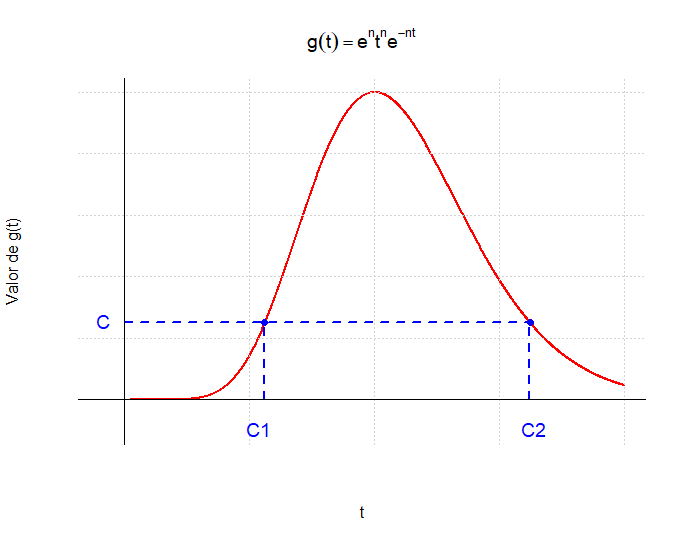
\includegraphics[scale=0.4]{figs/g_t.png}
    %\caption{Caption}
    \label{fig:enter-label}
\end{figure}

\end{block}
\end{frame}

\begin{frame}{}
\begin{block}{}
\justifying
Notem que $M_{X_{i}}(t)=(1-t\theta)^{-1},$ é a função geradora de momentos de $X_{i},~i=1,2,\ldots,n.$ Assim, a função geradora de momentos de $Y=2\Sumi X_{i}/\theta_0$ é dada por $M_{Y}(t)=(1-2t)^{-2n/2},$ que é a função geradora de momentos de uma variável $\chi^{2}(2n).$
\end{block}
\pause
\begin{block}{}
\justifying
Ou seja, $\Bar{X}/\theta_0 \leq c_1\SeSe Y=2\Sumi X_{i}/\theta_0\leq k_{1}=2nc_{1}$ ou 
\end{block}
\pause
\begin{block}{}
\justifying
$\Bar{X}/\theta_0 \geq c_2\SeSe Y=2\Sumi X_{i}/\theta_0\geq k_{2}=2nc_{2}$.
\end{block}
\end{frame}

\begin{frame}{}
\begin{block}{}
\justifying
Baseado nas observações anteriores, podemos utilizar a seguinte regra de decisão para o teste de nível $\alpha$:
\end{block}
\pause
\begin{block}{}
\justifying
Rejeitar $H_0$ se $(2/\theta_0) \sum_{i=1} X_i \leq \chi^2_{1-\alpha/2}(2n)$ ou $(2/\theta_0) \sum_{i=1} X_i \geq \chi^2_{\alpha/2}(2n),$
\end{block}
\begin{block}{}
\justifying
em que $\chi^2_{1-\alpha/2}(2n)$ é o quantil inferior $\alpha/2$ de uma distribuição $\chi^2$ com $2n$ graus de liberdade e $\chi^2_{\alpha/2}(2n)$ é o quantil superior $\alpha/2$ de uma distribuição $\chi^2$ com $2n$ graus de liberdade.
\end{block}
\end{frame}


\section{Teorema do Teste da Razão de Verossimilhança}
\begin{frame}{Teorema do Teste da Razão de Verossimilhança}
\begin{Teorema}
\justifying
Suponha que as condições de regularidade R0 a R5 são satisfeitas. Sob a hipótese nula, $H0: \theta = \theta_0,$ temos que $\{-2 \log \Lambda\} \ConvD \chi^2(1).$
\end{Teorema}
\pause
\begin{block}{Demonstração:}
\justifying
\textbf{Prova:} Expanda a função $\ell(\theta)$ em um Polinômio de Taylor em torno de $\theta_0$ de ordem 1 e avalie-a no estimador de máxima verossimilhança, $\hat{\theta}$. Isso resulta em
\begin{align}\label{6.3.8}
    \ell(\hat{\theta}) = \ell(\theta_{0}) + (\hat{\theta} - \theta_0)\ell'(\theta_{0}) + \frac{1}{2}(\hat{\theta} - \theta_0)^2 \ell''(\theta^{*}_{n}),
\end{align}
em que $\theta^*_n$ está entre $\hat{\theta}$ e $\theta_0.$
\end{block}
\end{frame}


\begin{frame}{}
\begin{block}{Demonstração:}
\justifying
Como $\hat{\theta} \ConvP \theta_0,$ segue que $\theta^*_n \ConvP \theta_0.$ Isso, além do fato de que a função $l'(\theta)$ é contínua e a equação (6.2.22) do Teorema 6.2.2 do livro texto (Hogg $8^{\circ}$ edição) implicam que
\begin{align}\label{6.3.9}
    -\frac{1}{n}\ell''(\theta^{*}_{n}) \ConvP I(\theta_0).
\end{align}

Pelo Corolário 6.2.3, do livro texto,

\begin{align}\label{6.3.10}
   \frac{1}{\sqrt{n}}\ell'(\theta_{0}) = \sqrt{n}(\hat{\theta} - \theta_0)I(\theta_0) + R_n, 
\end{align}

em que $R_n \ConvP 0.$ 

\end{block}
\end{frame}

\begin{frame}{}
\begin{block}{}
\justifying
Se substituirmos (\ref{6.3.9}) e (\ref{6.3.10}) na expressão (\ref{6.3.8}) e fizermos algumas simplificações, obtemos

\begin{align*}
    -2 \log \Lambda = 2(\ell(\hat{\theta}) - \ell(\theta_{0})) = \left[\sqrt{nI(\theta_0)}(\hat{\theta} - \theta_0)\right]^2 + R^*_n,
\end{align*}
em que $R^*_n \ConvP 0.$ Pelo Teorema 5.2.4 e pelo Teorema 6.2.2, o primeiro termo no lado direito da equação acima converge em distribuição para uma distribuição $\chi^2$ com um grau de liberdade. $\cqd$
\end{block}
\end{frame}

\begin{frame}{}
\begin{block}{}
\justifying
Logo, defina a estatística de teste $\chi^2_L = -2 \log \Lambda.$ Para as hipóteses, 
\[ H_0 : \theta = \theta_0 \quad \text{versus} \quad H_1 : \theta \neq \theta_0, \]

este teorema sugere a regra de decisão:
\[
\text{Rejeitar } H0 \text{ em favor de } H1 \text{ se } \chi^2_L \geq \chi^2_\alpha(1).
\]

Pelo último teorema, este teste possui nível assintótico $\alpha.$ Se não conseguirmos obter a estatística de teste ou sua distribuição em uma forma fechada, podemos usar este teste assintótico.
\end{block}
\end{frame}

\section{Teste do Tipo Wald}
\begin{frame}{Teste do Tipo Wald}
\begin{block}{}
\justifying
Além do teste da razão de verossimilhança, na prática, são empregados outros dois testes relacionados à verossimilhança. Uma estatística de teste natural é baseada na distribuição assintótica de $\hat{\theta}$. Considere a estatística
\begin{align*}
    \chi^2_W = \left\{\sqrt{nI(\hat{\theta})}(\hat{\theta} - \theta_0)\right\}^2.
\end{align*}

como $I(\theta)$ é uma função contínua, $I(\hat{\theta}) \ConvP I(\theta_0)$ sob a hipótese nula. Portanto, sob $H0, \chi^2_W$ possui uma distribuição assintótica $\chi^2$ com um grau de liberdade. 
\end{block}
\pause
\begin{block}{}
\justifying
Isso sugere a regra de decisão
\begin{align}\label{6.3.14}
    \text{Rejeitar } H0 \text{ em favor de } H1 \text{ se } \chi^2_W \geq \chi^2_\alpha(1).
\end{align}

Este teste também possui nível assintótico $\alpha.$
\end{block}
\end{frame}

\begin{frame}{}
\begin{block}{}
\begin{tabular}{cl}  
         \begin{tabular}{c}
           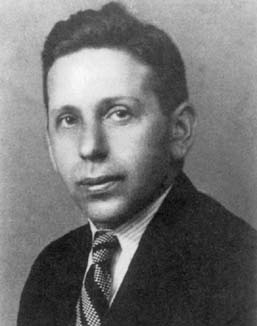
\includegraphics[height=5cm, width=3.5cm]{figs/Abraham_Wald.jpg}
           \end{tabular}
           & \begin{tabular}{l}
             \parbox{0.5\linewidth}{O teste (\ref{6.3.14}) é frequentemente referido como um teste do tipo Wald, em homenagem a \textbf{Abraham Wald} (nasceu em 31 de outubro de 1902, morreu em 1950 de acidente de avião), que foi um estatístico do século XX. Após sua morte, Wald foi criticado por Sir Ronald A. Fisher. O trabalho de Wald foi defendido, posteriormente, por Jerzy Neyman e outros acadêmicos proeminentes.   
    }
         \end{tabular}  \\
\end{tabular}

\end{block}
\end{frame}

\section{Teste do Tipo Escore}
\begin{frame}{Teste do Tipo Escore}
\begin{block}{}
\begin{tabular}{rl}  
\begin{tabular}{r}
\parbox{0.5\linewidth}{O terceiro teste é chamado de teste de escores de Rao, em homenagem a \textbf{Calyampudi Radhakrishna Rao}(10 de setembro de 1920 - 22 de agosto de 2023). A American Statistical Association o descreveu como ``uma lenda viva cujo trabalho influenciou não apenas as estatísticas, mas teve implicações de longo alcance para diversos outros campos.'' O Times of India listou Rao como um dos 10 maiores cientistas indianos de todos os tempos.   
    }
\end{tabular}
&   
\begin{tabular}{l}
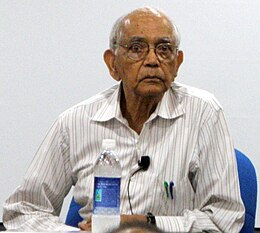
\includegraphics[height=5cm, width=3.5cm]{figs/CRRao.JPG}
\end{tabular}\\           
\end{tabular}
 
\end{block}
\end{frame}

\begin{frame}{}
\begin{block}{}
\justifying
Os escores são os componentes do vetor
\[
S(\theta) = \left\{\frac{\partial \log f(X_1; \theta)}{\partial \theta}, \ldots, \frac{\partial \log f(X_n; \theta)}{\partial \theta}\right\}.
\]

Em nossa notação, temos
\[
\frac{1}{\sqrt{n}}\ell'(\theta_{0}) = \frac{1}{\sqrt{n}}\Sumi \frac{\partial \log f(X_i; \theta_0)}{\partial \theta}.
\]
\end{block}
\end{frame}

\begin{frame}{}
\begin{block}{}
\justifying
Defina a estatística
\[
\chi^2_R = \left\{\frac{\ell'(\theta_{0})}{\sqrt{nI(\theta_0)}}\right\}^2. 
\]

Sob H0, segue da expressão (\ref{6.3.10}) que
\[
\chi^2_R = \chi^2_W + R_{0n},
\]
em que $R_{0n}$ converge para $0$ em probabilidade. Portanto, a próxima regra de decisão define um teste.
\end{block}
\pause
\begin{block}{}
\justifying
\begin{align}\label{6.3.20}
    \text{Rejeite } H0 \text{ em favor de } H1 \text{ se } \chi^2_R \geq \chi^2_\alpha(1).
\end{align}
\end{block}
\end{frame}

\section{Exemplos TRV, Wald e Escore}
\begin{frame}{Exemplos TRV, Wald e Escore}
\begin{block}{}
\justifying
Seja \(X_1, \ldots, X_n\) uma amostra aleatória com uma distribuição beta(\(\theta, 1\)). Considere as hipóteses: 

$$H_0: \theta = 1~ \text{versus}~ H_1: \theta \neq 1$$
\end{block}
\pause

\begin{block}{}
A densidade da Beta\((\theta, 1)\) é:
\[
f(x; \theta) = \theta x^{\theta - 1}, \quad 0 < x < 1, \quad \theta > 0.
\]

O logaritmo da densidade, que chamaremos de \(\ell(\theta)\), é:
\[
\ell(\theta) = \log f(x; \theta) = \log \theta + (\theta - 1) \log x.
\]

\end{block}
\end{frame}

\begin{frame}
\begin{block}{}
	\justifying
	É possível mostrar que \(\hat{\theta} = -\frac{n}{\Sumi \log X_i}\) é o estimador de máxima verossimilhança de \(\theta\). Após alguma simplificação, o valor da função de verossimilhança no estimador de máxima verossimilhança é dado por:
	
	\[L(\hat{\theta}) = \left(- \sum_{i=1}^n \log X_i\right)^{-n}\exp\left\{n(\log n - 1) - \sum_{i=1}^n \log X_i\right\}.\] 
\end{block}
\end{frame}

\begin{frame}{Exemplos TRV, Wald e Escore}
\begin{block}{}
\justifying
Além disso, \(L(1) = 1\), portanto, a estatística do teste da razão de verossimilhança é \(\Lambda = \frac{1}{L(\hat{\theta})}\), de modo que:

{\small
\[\chi^2_L = -2 \log \Lambda = 2\left(- \sum_{i=1}^n \log X_i - n \log\left(-\sum_{i=1}^n \log X_i\right) - n + n \log n\right)\]
}

Lembre-se de que a informação para esta distribuição é \(I(\theta) = \theta^{-2}\). 
\end{block}
\end{frame}

\begin{frame}{Exemplos TRV, Wald e Escore}
\begin{block}{}
\justifying
Para o teste do tipo Wald, podemos estimar isso consistentemente como \(\hat{\theta}^{-2}\). O teste do tipo Wald simplifica-se para:

\[\chi^2_W = \sqrt{\dfrac{n}{\hat{\theta}^{2}}}(\hat{\theta}-1)=n\left(1 - \frac{1}{\hat{\theta}}\right)^2\]
\end{block}
\end{frame}


\begin{frame}{Exemplos TRV, Wald e Escore}
\begin{block}{}
\justifying
Por fim, para o teste do tipo escores, \(\ell'(1)\) é dado por:

\[\ell'(1) = \sum_{i=1}^n \log X_i + n\]

Portanto, a estatística do teste do tipo escores é:

\[\chi^2_R = \left\{\dfrac{\left(\Sumi \log X_i + n\right)}{\sqrt{n}}\right\}^{2}.\]
\end{block}
\end{frame}

\section{Conexão entre os Três Testes}
\begin{frame}
	\begin{block}{}
\justifying		
		Os testes de Razão de Verossimilhança (LRT), Wald e Escore avaliam a mesma hipótese nula, mas de formas distintas:
		
		\begin{itemize}
			\justifying
			\item \textbf{Razão de Verossimilhança (LRT):} Compara o ajuste de dois modelos, um com e outro sem restrições, por meio da razão das verossimilhanças.\pause
			\item \textbf{Wald:} Avalia diretamente se o parâmetro estimado está próximo do valor hipotético, utilizando a variância do estimador.\pause
			\item \textbf{Escore:} Analisa o gradiente da verossimilhança no ponto nulo para identificar evidências de desvio em direção à alternativa.
		\end{itemize}
	\end{block}
\end{frame}

\begin{frame}
	\begin{block}{}
		\justifying
		Os três testes têm como base a função de verossimilhança, mas fazem uso de diferentes aspectos da mesma:
		\begin{itemize}
			\justifying
			\item O \textbf{LRT} considera a \textit{diferença máxima} na função de verossimilhança entre os modelos nulo e alternativo.\pause
			\item O \textbf{teste de Wald} utiliza a \textit{distância do estimador} ao valor nulo ponderada pela variância.\pause
			\item O \textbf{teste de escore} analisa o \textit{declive da verossimilhança} no ponto nulo.
		\end{itemize}
	\end{block}
\end{frame}

\begin{frame}
	\begin{block}{}
		\begin{itemize}
			\justifying
			\item \textbf{Teste de Wald:} 
			\begin{itemize}
				\justifying
				\item Fácil de implementar, pois depende apenas do estimador de máxima verossimilhança (EMV) e de sua variância estimada.\pause
				\item Pode ser impreciso em pequenas amostras ou quando o parâmetro está próximo da borda do espaço paramétrico.\pause
			\end{itemize}
			\item \textbf{Teste de Razão de Verossimilhança (LRT):}
			\begin{itemize}
				\justifying
				\item Considerado mais robusto, pois avalia a qualidade do ajuste entre os modelos nulo e alternativo.\pause
				\item Pode ser computacionalmente caro, já que exige a estimação do modelo sob a hipótese alternativa.\pause
			\end{itemize}
			\item \textbf{Teste de Escore:}
			\begin{itemize}
				\justifying
				\item Útil quando a estimação do modelo alternativo é difícil, pois depende apenas das derivadas da verossimilhança no ponto nulo.\pause
				\item Assume que o modelo nulo está bem especificado, o que pode limitar sua aplicabilidade.
			\end{itemize}
		\end{itemize}
	\end{block}
\end{frame}

\begin{frame}{\Home}
\begin{block}{}
\justifying
\begin{itemize}
    \item \textbf{Exercícios da seção 6.3:} 6, 9, 10, 11, 12, 13, 16, 18, 19.
\end{itemize}
\end{block}
\nocite{hogg}
\end{frame}

\begin{frame}[allowframebreaks]
\frametitle{\bf Referências}
\printbibliography
\end{frame}


\end{document}



\begin{frame}{}
\begin{block}{}
\justifying

\end{block}
\end{frame}

\begin{frame}{}
\begin{block}{}
\justifying

\end{block}
\end{frame}

\begin{frame}{}
\begin{block}{}
\justifying

\end{block}
\end{frame}


\begin{frame}{}
\begin{block}{}
\justifying

\end{block}
\end{frame}

\begin{frame}{}
\begin{block}{}
\justifying

\end{block}
\end{frame}


\begin{frame}{}
\begin{block}{}
\justifying

\end{block}
\end{frame}

\begin{frame}{}
\begin{block}{}
\justifying

\end{block}
\end{frame}


\begin{frame}{}
\begin{block}{}
\justifying

\end{block}
\end{frame}

\begin{frame}{}
\begin{block}{}
\justifying

\end{block}
\end{frame}

\begin{frame}{}
\begin{block}{}
\justifying

\end{block}
\end{frame}


\begin{frame}{}
\begin{block}{}
\justifying

\end{block}
\end{frame}

\begin{frame}{}
\begin{block}{}
\justifying

\end{block}
\end{frame}


\begin{frame}{}
\begin{block}{}
\justifying

\end{block}
\end{frame}

\begin{frame}{}
\begin{block}{}
\justifying

\end{block}
\end{frame}


\begin{frame}{}
\begin{block}{}
\justifying

\end{block}
\end{frame}

\begin{frame}{}
\begin{block}{}
\justifying

\end{block}
\end{frame}

\begin{frame}{}
\begin{block}{}
\justifying

\end{block}
\end{frame}

\begin{frame}{}
\begin{block}{}
\justifying

\end{block}
\end{frame}


\begin{frame}{}
\begin{block}{}
\justifying

\end{block}
\end{frame}

\begin{frame}{}
\begin{block}{}
\justifying

\end{block}
\end{frame}

\begin{frame}{}
\begin{block}{}
\justifying

\end{block}
\end{frame}


\begin{frame}{}
\begin{block}{}
\justifying

\end{block}
\end{frame}

\begin{frame}{}
\begin{block}{}
\justifying

\end{block}
\end{frame}


\begin{frame}{}
\begin{block}{}
\justifying

\end{block}
\end{frame}

\begin{frame}{}
\begin{block}{}
\justifying

\end{block}
\end{frame}


\begin{frame}{}
\begin{block}{}
\justifying

\end{block}
\end{frame}

\begin{frame}{}
\begin{block}{}
\justifying

\end{block}
\end{frame}

\begin{frame}{}
\begin{block}{}
\justifying

\end{block}
\end{frame}


\begin{frame}{}
\begin{block}{}
\justifying

\end{block}
\end{frame}

\begin{frame}{}
\begin{block}{}
\justifying

\end{block}
\end{frame}


\begin{frame}{}
\begin{block}{}
\justifying

\end{block}
\end{frame}

\begin{frame}{}
\begin{block}{}
\justifying

\end{block}
\end{frame}


\begin{frame}{}
\begin{block}{}
\justifying

\end{block}
\end{frame}

\begin{frame}{}
\begin{block}{}
\justifying

\end{block}
\end{frame}

\begin{frame}{}
\begin{block}{}
\justifying

\end{block}
\end{frame}


\begin{frame}{}
\begin{block}{}
\justifying

\end{block}
\end{frame}

\begin{frame}{}
\begin{block}{}
\justifying

\end{block}
\end{frame}


\begin{frame}{}
\begin{block}{}
\justifying

\end{block}
\end{frame}

\begin{frame}{}
\begin{block}{}
\justifying

\end{block}
\end{frame}


\begin{frame}{}
\begin{block}{}
\justifying

\end{block}
\end{frame}

\begin{frame}{}
\begin{block}{}
\justifying

\end{block}
\end{frame}

\begin{frame}{}
\begin{block}{}
\justifying

\end{block}
\end{frame}


\begin{frame}{}
\begin{block}{}
\justifying

\end{block}
\end{frame}

\begin{frame}{}
\begin{block}{}
\justifying

\end{block}
\end{frame}


\begin{frame}{}
\begin{block}{}
\justifying

\end{block}
\end{frame}

\begin{frame}{}
\begin{block}{}
\justifying

\end{block}
\end{frame}


\begin{frame}{}
\begin{block}{}
\justifying

\end{block}
\end{frame}

\begin{frame}{}
\begin{block}{}
\justifying

\end{block}
\end{frame}

\begin{frame}{}
\begin{block}{}
\justifying

\end{block}
\end{frame}


\begin{frame}{}
\begin{block}{}
\justifying

\end{block}
\end{frame}

\begin{frame}{}
\begin{block}{}
\justifying

\end{block}
\end{frame}


\begin{frame}{}
\begin{block}{}
\justifying

\end{block}
\end{frame}

\begin{frame}{}
\begin{block}{}
\justifying

\end{block}
\end{frame}


\begin{frame}{}
\begin{block}{}
\justifying

\end{block}
\end{frame}

\begin{frame}{}
\begin{block}{}
\justifying

\end{block}
\end{frame}

\begin{frame}{}
\begin{block}{}
\justifying

\end{block}
\end{frame}


\begin{frame}{}
\begin{block}{}
\justifying

\end{block}
\end{frame}

\begin{frame}{}
\begin{block}{}
\justifying

\end{block}
\end{frame}


\begin{frame}{}
\begin{block}{}
\justifying

\end{block}
\end{frame}

\begin{frame}{}
\begin{block}{}
\justifying

\end{block}
\end{frame}


\begin{frame}{}
\begin{block}{}
\justifying

\end{block}
\end{frame}

\begin{frame}{}
\begin{block}{}
\justifying

\end{block}
\end{frame}

\begin{frame}{}
\begin{block}{}
\justifying

\end{block}
\end{frame}


\begin{frame}{}
\begin{block}{}
\justifying

\end{block}
\end{frame}

\begin{frame}{}
\begin{block}{}
\justifying

\end{block}
\end{frame}




\begin{frame}{}
\begin{block}{}
\justifying

\end{block}
\end{frame}


\begin{frame}{}
\begin{block}{}
\justifying

\end{block}
\end{frame}

\begin{frame}{}
\begin{block}{}
\justifying

\end{block}
\end{frame}

\begin{frame}{}
\begin{block}{}
\justifying

\end{block}
\end{frame}


\begin{frame}{}
\begin{block}{}
\justifying

\end{block}
\end{frame}

\begin{frame}{}
\begin{block}{}
\justifying

\end{block}
\end{frame}